\documentclass[nogin, 10pt]{article}
\usepackage{natbib}
\usepackage[english]{babel}
\usepackage[latin1]{inputenc}
\usepackage[colorlinks = true]{hyperref}
\usepackage{bbm, amssymb, amsmath, amsthm}
\usepackage[T1]{fontenc} 
\usepackage{aeguill, fancyhdr, latexsym, mathrsfs, verbatim, colortbl}
\usepackage[a4paper,
            inner=30mm,
            outer=40mm,
            top=40mm,
            bottom=40mm,
            marginparwidth=30mm,
            marginparsep=5mm]{geometry}
\usepackage{tikz}
\usepackage{Sweave}


\setlength{\parindent}{0pt}
\setlength{\parskip}{1.3ex}

\begin{document}
	
	Here we created a function we never got around to using.
\begin{Schunk}
\begin{Sinput}
> 	x<-seq(-10,10,0.1)
> 	a<-sapply(x,dnorm,-1,1)
> 	b<-sapply(x,dnorm,0,2)
> 	c<-sapply(x,dnorm,2,3)
\end{Sinput}
\end{Schunk}
Create an x which we plug into \texttt{dnorm} so we can plot it later.

\begin{Schunk}
\begin{Sinput}
> 	print(qplot(x,a)+geom_line()+ylab("y")) #gaussian with (-1,1)
> 	print(qplot(x,b)+geom_line()+ylab("y")) #gaussian with (0,2)
> 	print(qplot(x,c)+geom_line()+ylab("y")) #gaussian with (2,3)
\end{Sinput}
\end{Schunk}
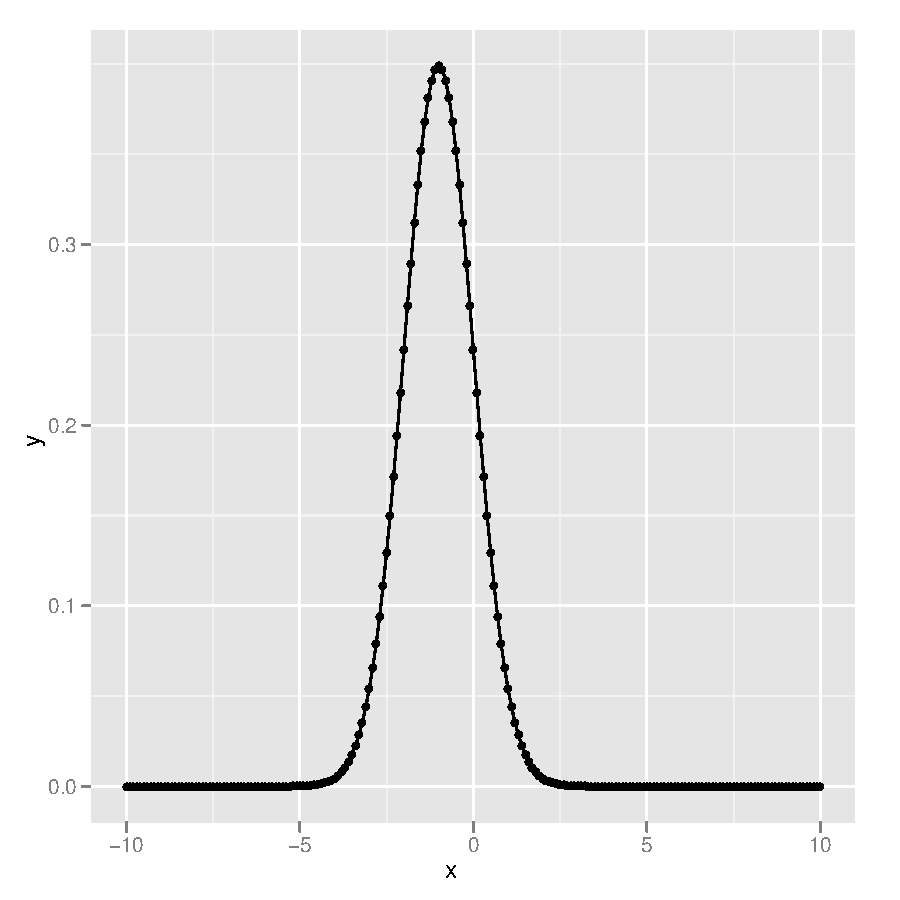
\includegraphics{Sweave-003}
A bunch of gaussian plots. Unto question 2!

\begin{Schunk}
\begin{Sinput}
> 	#q2: make a 2d-gaussian with N=100
> 	N=100
> 	twoDgauss<-function(N,mu,sig11,sig12,sig21,sig22){
+ 	  #assumes mean is (mu,mu)
+ 	  z<-matrix(c(rnorm(N*2)),2,N)
+ 	  mu<-matrix(replicate(N,mu),2,N)
+ 	  sigma<-matrix(c(sig11,sig12,sig21,sig22),2,2)
+ 	  L<-t(chol(sigma))
+ 	  y<-mu+(L%*%z)
+ 	  return(y)
+ 	}
> 	y<-twoDgauss(N=N,mu=1,sig11=0.3,sig12=0.2,sig21=0.2,sig22=0.2)
> 	y10k<-twoDgauss(N=10000,mu=1,sig11=0.3,sig12=0.2,sig21=0.2,sig22=0.2)
\end{Sinput}
\end{Schunk}
We defined a function that spits out gaussian stuff given $\Sigma$ and $\mu$.
\begin{Schunk}
\begin{Sinput}
> 	print(qplot(y[1,],y[2,])+xlab("x")+ylab("y"))
> 	print(qplot(y10k[1,],y10k[2,])+geom_bin2d(aes(fill=log2(..count..)),binwidth=c(0.05,0.05))+xlab("x")+ylab("y"))
\end{Sinput}
\end{Schunk}
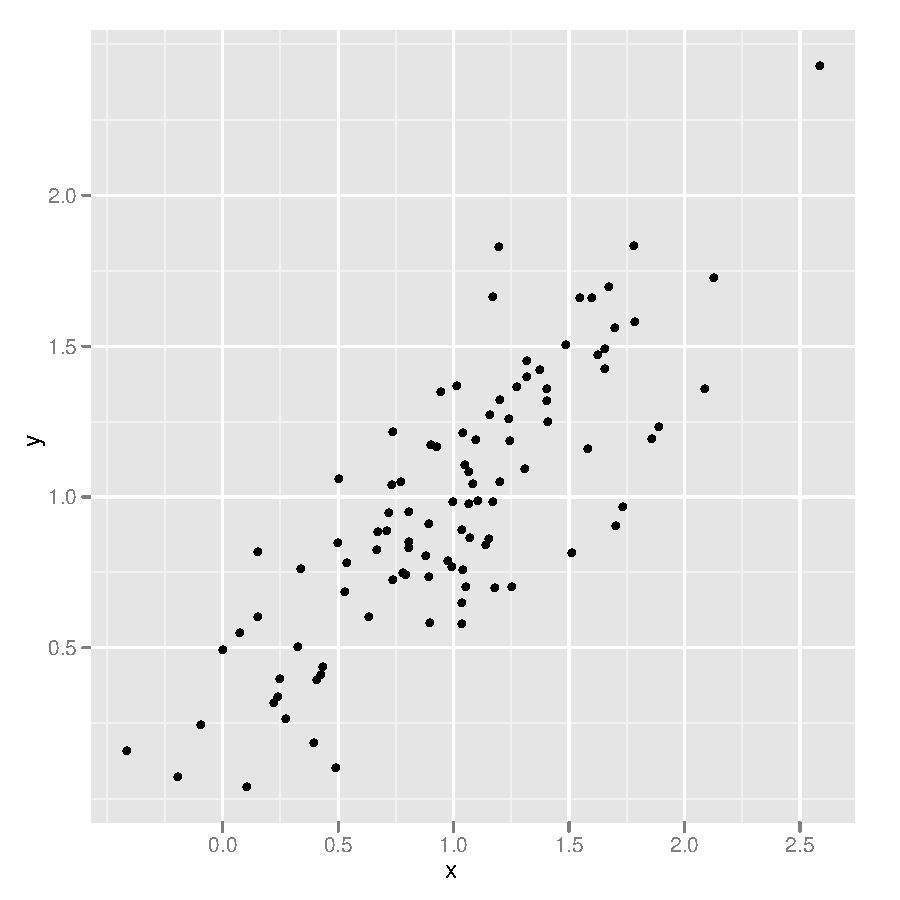
\includegraphics{Sweave-005}
Some of the 2D Gaussian plots.
\end{document}



